\documentclass[runningheads]{llncs}

\usepackage[T1]{fontenc}
\usepackage[utf8]{inputenc}
\usepackage{graphicx}
\usepackage{amsmath,amssymb,amsfonts}
\usepackage{booktabs}
\usepackage{array}
\usepackage{float}
\usepackage{xcolor}
\usepackage{hyperref}

\hypersetup{
    colorlinks=true,
    linkcolor=blue!60!black,
    citecolor=blue!60!black,
    urlcolor=blue!60!black
}
\renewcommand\UrlFont{\color{blue}\rmfamily}
\urlstyle{rm}

\begin{document}

\title{Investiga\c{c}\~{a}o Emp\'{i}rica, Conex\~{o}es Residuais e Mecanismos de Aten\c{c}\~{a}o em Redes Neurais Convolucionais para Classifica\c{c}\~{a}o no CIFAR-10}
\titlerunning{Relat\'{o}rio T\'{e}cnico de Arquitetura: Reprodu\c{c}\~{a}o e Modifica\c{c}\~{o}es em CNN}

\author{Jos\'{e} Alb\'{e}rico Rocha da Silva\inst{1}}
\authorrunning{J. A. R. da Silva}

\institute{Universidade Federal Rural de Pernambuco (UFRPE)\\
Departamento de Computa\c{c}\~{a}o -- T\'{o}picos Avan\c{c}ados em Intelig\^{e}ncia Artificial (2026.2)\\
Recife - PE, Brasil\\
\email{jose.alberico@ufrpe.br}\\
\url{https://github.com/albericolx/Topicos_Avancados_IA}}

\maketitle

\begin{abstract}
Este artigo cient\'{i}fico comparativo formaliza o cumprimento do Artefato \texttt{[5] arquitetura tech report} (\texttt{arq$\cdot$p}) da disciplina T\'{o}picos Avan\c{c}ados em Intelig\^{e}ncia Artificial (UFRPE 2026.2). O estudo documenta a reprodu\c{c}\~{a}o rigorosa e a subsequente extens\~{a}o arquitetural de uma rede neural convolucional moderna baseada na literatura acad\^{e}mica recente (\textit{Dizabadi, arXiv:2604.23861, 2026}). A arquitetura de refer\^{e}ncia compreende 6 camadas convolucionais organizadas em tr\^{e}s blocos duplos intercalados por normaliza\c{c}\~{a}o em lote (\textit{Batch Normalization}), \textit{Max Pooling} e \textit{Dropout} progressivo, totalizando exatamente $552.874$ par\^{a}metros. A partir do diagn\'{o}stico de instabilidade por desvanecimento de gradientes em profundidades elevadas e de sobreajuste severo identificado no artigo de origem, formulam-se e implementam-se tr\^{e}s modifica\c{c}\~{o}es in\'{e}ditas: (1) Conex\~{o}es Residuais aditivas (\textit{Residual Skip Connections}) estilo ResNet; (2) Protocolo de regulariza\c{c}\~{a}o estoc\'{a}stica por \textit{Data Augmentation} em tempo real (\textit{Random Crop} com preenchimento reflexivo e \textit{Random Horizontal Flip}); e (3) Mecanismo de Aten\c{c}\~{a}o de Canal \textit{Squeeze-and-Excitation} (\textit{SE-Block}), culminando na s\'{i}ntese de um Modelo Combinado integrado. Conduziu-se um estudo de abla\c{c}\~{a}o sistem\'{a}tico sobre uma parti\c{c}\~{a}o estratificada sem vazamento (\textit{zero-leakage}) do \textit{benchmark} can\^{o}nico CIFAR-10 ($25.000$ amostras de treino e $5.000$ de teste). Apresenta-se uma matriz comparativa rigorosa confrontando as m\'{e}tricas reportadas pelos autores originais, as reproduzidas pelo estudante e as p\'{o}s-modifica\c{c}\~{o}es, al\'{e}m de uma an\'{a}lise qualitativa detalhada com inspe\c{c}\~{a}o visual das inst\^{a}ncias cr\'{i}ticas de confus\~{a}o entre categorias sem\^{a}nticas pr\'{o}ximas.

\keywords{Redes Neurais Convolucionais \and Conex\~{o}es Residuais \and Squeeze-and-Excitation \and Data Augmentation \and CIFAR-10 \and Estudo de Abla\c{c}\~{a}o.}
\end{abstract}

% ============================================================================
\section{Introdu\c{c}\~{a}o, Artigo Base Selecionado e Hip\'{o}teses de Contribui\c{c}\~{a}o}
\label{sec:intro}
% ============================================================================

\subsection{Escolha Fundamentada do Artigo Acad\^{e}mico de Refer\^{e}ncia}
O desenvolvimento de arquiteturas de aprendizado profundo para vis\~{a}o computacional atingiu expressivo amadurecimento emp\'{i}rico na \'{u}ltima d\'{e}cada. Todavia, a compreens\~{a}o fina das intera\c{c}\~{o}es entre profundidade da rede, regulariza\c{c}\~{a}o estoc\'{a}stica e fluxo de gradientes permanece como um t\'{o}pico central de investiga\c{c}\~{a}o experimental. Em conson\^{a}ncia com os requisitos de sele\c{c}\~{a}o da disciplina (artigo acad\^{e}mico $\ge 2023$, c\'{o}digo aberto e topologia moderna de aprendizado profundo), selecionou-se como base anal\'{i}tica o trabalho de Dizabadi (2026)~\cite{dizabadi2026empirical}:
\begin{quote}
    \textbf{Artigo de Refer\^{e}ncia:} Dizabadi, N. K. \textit{``Empirical Ablation and Ensemble Optimization of a Convolutional Neural Network for CIFAR-10 Classification''}, arXiv:2604.23861v1, Abril de 2026.
\end{quote}

O artigo selecionado disponibiliza de forma transparente e integral o c\'{o}digo-fonte e a metodologia experimental desenvolvida sobre o conjunto can\^{o}nico CIFAR-10~\cite{krizhevsky2009learning}. O modelo can\^{o}nico proposto pelos autores consiste em uma rede convolucional de $6$ camadas agrupadas em pares de convolu\c{c}\~{a}o com filtros $3 \times 3$, intercaladas por camadas de Normaliza\c{c}\~{a}o em Lote (\textit{Batch Normalization})~\cite{ioffe2015batch}, ativa\c{c}\~{a}o ReLU, subamostragem por \textit{Max Pooling} $2 \times 2$ e regulariza\c{c}\~{a}o por \textit{Dropout}~\cite{srivastava2014dropout}:
\begin{itemize}
    \item \textbf{Bloco Convolucional 1:} $\text{Conv2D}(3 \to 32, 3 \times 3) + \text{BN} + \text{ReLU} + \text{Conv2D}(32 \to 32, 3 \times 3) + \text{BN} + \text{ReLU} + \text{MaxPool}(2 \times 2) + \text{Dropout}(0{,}30)$.
    \item \textbf{Bloco Convolucional 2:} $\text{Conv2D}(32 \to 64, 3 \times 3) + \text{BN} + \text{ReLU} + \text{Conv2D}(64 \to 64, 3 \times 3) + \text{BN} + \text{ReLU} + \text{MaxPool}(2 \times 2) + \text{Dropout}(0{,}50)$.
    \item \textbf{Bloco Convolucional 3:} $\text{Conv2D}(64 \to 128, 3 \times 3) + \text{BN} + \text{ReLU} + \text{Conv2D}(128 \to 128, 3 \times 3) + \text{BN} + \text{ReLU} + \text{MaxPool}(2 \times 2) + \text{Dropout}(0{,}50)$.
    \item \textbf{Classificador Denso:} $\text{Flatten}(128 \times 4 \times 4 = 2048) \to \text{Linear}(2048 \to 128) + \text{ReLU} + \text{BN} + \text{Dropout}(0{,}50) \to \text{Linear}(128 \to 10)$.
\end{itemize}
Essa topologia computacional totaliza exatamente \textbf{$552.874$ par\^{a}metros} ($551.722$ par\^{a}metros trein\'{a}veis e $1.152$ estat\'{i}sticas correntes de \textit{running mean/var} do Batch Normalization).

\subsection{Motiva\c{c}\~{a}o Te\'{o}rica e Diagn\'{o}stico de Lacunas}
No estudo original de Dizabadi~\cite{dizabadi2026empirical}, os autores exploraram $17$ varia\c{c}\~{o}es emp\'{i}ricas cobrindo taxas de aprendizado, fam\'{i}lias de otimizadores (SGD com momentum, RMSprop, Adam), dropout adaptativo e combina\c{c}\~{o}es de \textit{ensembles} homog\^{e}neos. N\~{a}o obstante, a an\'{a}lise cr\'{i}tica do texto e dos registros quantitativos revela duas vulnerabilidades estruturais expressivas:
\begin{enumerate}
    \item \textbf{Instabilidade e Colapso em Profundidade Elevada:} No experimento denominado \textit{Step 11}, ao estender a arquitetura de $6$ para $8$ camadas convolucionais consecutivas, a acur\'{a}cia de teste colapsou de $83{,}42\%$ para $70{,}66\%$. Os autores atribu\'{i}ram esse decl\'{i}nio ao fen\^{o}meno cl\'{a}ssico de desvanecimento de gradientes (\textit{vanishing gradients}) decorrente do encadeamento estrito de operadores lineares e ativa\c{c}\~{o}es sucessivas, mas abstiveram-se de implementar conex\~{o}es de atalho de fluxo (\textit{skip connections}).
    \item \textbf{Aus\^{e}ncia de Aumento de Dados e Sobreajuste:} O protocolo de treino do artigo base alimentou os modelos estritamente com imagens est\'{a}ticas sem qualquer perturba\c{c}\~{a}o espacial estoc\'{a}stica, gerando uma discrep\^{a}ncia severa entre o desempenho no treino ($> 95\%$) e no teste ($\approx 83\%$).
    \item \textbf{Pondera\c{c}\~{a}o Uniforme de Canais:} As convolu\c{c}\~{o}es padr\~{a}o operam sob o pressuposto impl\'{i}cito de que todos os mapas de caracter\'{i}sticas gerados em um bloco contribuem igualmente para a discrimina\c{c}\~{a}o supervisionada, sem moduladores de sali\^{e}ncia intra-canal.
\end{enumerate}

\subsection{Hip\'{o}teses Formais de Contribui\c{c}\~{a}o}
Com o prop\'{o}sito de sanar tais lacunas de forma in\'{e}dita frente \`{a}s $17$ etapas do artigo original, formulam-se tr\^{e}s hip\'{o}teses de pesquisa:
\begin{itemize}
    \item \textbf{Hip\'{o}tese 1 ($H_1$ -- Conex\~{o}es Residuais):} A introdu\c{c}\~{a}o de atalhos aditivos de identidade $\mathbf{y} = \sigma(\mathcal{F}(\mathbf{x}) + \mathbf{x})$ nos blocos convolucionais garante um canal direto para a propaga\c{c}\~{a}o dos gradientes de erro sem atenua\c{c}\~{a}o exponencial, estabilizando o aprendizado e elevando a efic\'{a}cia da converg\^{e}ncia sem exigir explos\~{a}o param\'{e}trica.
    \item \textbf{Hip\'{o}tese 2 ($H_2$ -- Data Augmentation Estoc\'{a}stico):} A perturba\c{c}\~{a}o estoc\'{a}stica din\^{a}mica no espa\c{c}o de pixels (recortes aleat\'{o}rios de $32 \times 32$ com \textit{padding} e espelhamento horizontal) imp\~{o}e invari\^{a}ncia translacional e reflexiva \`{a}s representaciones latentes, reduzindo o sobreajuste e estreitando o fosso de generaliza\c{c}\~{a}o.
    \item \textbf{Hip\'{o}tese 3 ($H_3$ -- Mecanismo de Aten\c{c}\~{a}o Squeeze-and-Excitation):} A recalibra\c{c}\~{a}o din\^{a}mica dos mapas de ativa\c{c}\~{a}o mediante compress\~{a}o espacial global (\textit{squeeze}) e depend\^{e}ncia inter-canais n\~{a}o-linear (\textit{excitation}) permite \`{a} rede priorizar canais ricos em padr\~{o}es morfol\'{o}gicos e suprimir ru\'{i}dos de fundo com custo computacional marginal ($< 1\%$ de par\^{a}metros).
\end{itemize}

% ============================================================================
\section{Trabalhos Relacionados}
\label{sec:related}
% ============================================================================

\subsection{Evolu\c{c}\~{a}o das CNNs Can\^{o}nicas e a Quebra do Paradigma Residual}
A consolida\c{c}\~{a}o das redes neurais convolucionais como arquitetura dominante para vis\~{a}o computacional remonta \`{a} introdu\c{c}\~{a}o da AlexNet e ao refinamento sistem\'{a}tico proposto pelas redes VGG de Simonyan e Zisserman~\cite{simonyan2014very}, as quais demonstraram que a substitui\c{c}\~{a}o de filtros amplos por cascata de n\'{u}cleos diminutos de $3 \times 3$ amplia a capacidade n\~{a}o-linear do modelo mantendo o campo receptivo efetivo. Contudo, \`{a} medida que as arquiteturas ultrapassaram uma dezena de camadas empilhadas, a literatura deparou-se com o obst\'{a}culo da degrada\c{c}\~{a}o de aprendizado: contra-intuitivamente, redes substancialmente mais profundas passaram a registrar erros de treinamento superiores \`{a}s suas contrapartes mais rasas, patologia desacoplada de sobreajuste. Esse dilema foi formalmente superado pelo trabalho seminal de He et al.~\cite{he2016deep} com as \textit{Deep Residual Networks} (ResNet). Ao reformular o mapeamento objetivo subjacente $\mathcal{H}(\mathbf{x})$ como um res\'{i}duo aditivo $\mathcal{F}(\mathbf{x}) = \mathcal{H}(\mathbf{x}) - \mathbf{x}$, os autores habilitaram que o gradiente da fun\c{c}\~{a}o de custo $\mathcal{L}$ seja retropropagado diretamente conforme $\frac{\partial \mathcal{L}}{\partial \mathbf{x}} = \frac{\partial \mathcal{L}}{\partial \mathbf{y}} \left(\frac{\partial \mathcal{F}}{\partial \mathbf{x}} + \mathbf{I}\right)$. A presen\c{c}\~{a}o da matriz identidade $\mathbf{I}$ impede que o sinal de erro convirja assintoticamente a zero mesmo quando os pesos das camadas convolucionais transitam por magnitudes pr\'{o}ximas de zero, solvendo a barreira que levou ao colapso do Step 11 no estudo de Dizabadi~\cite{dizabadi2026empirical}.

\subsection{Mecanismos de Aten\c{c}\~{a}o e Recalibra\c{c}\~{a}o Din\^{a}mica de Canais}
Paralelamente \`{a}s inova\c{c}\~{o}es no fluxo de conectividade residual, a comunidade de vis\~{a}o computacional passou a questionar a premissa de invari\^{a}ncia e equipondera\c{c}\~{a}o entre os m\'{u}ltiplos canais convolucionais. Tradicionalmente, o operador convolucional agrega informa\c{c}\~{o}es espaciais e inter-canais de forma indiferenciada ao longo do tensor de volume $\mathbf{U} \in \mathbb{R}^{H \times W \times C}$. Visando dotar os modelos da capacidade de modular a relev\^{a}ncia sem\^{a}ntica de cada canal, Hu et al.~\cite{hu2018squeeze} propuseram as redes \textit{Squeeze-and-Excitation} (SENet), que conquistaram a \'{u}ltima edi\c{c}\~{a}o do desafio ImageNet ILSVRC. A arquitetura SE introduz uma opera\c{c}\~{a}o de compress\~{a}o espacial global (\textit{Global Average Pooling}) que resume a dispers\~{a}o de cada canal em um escalar estat\'{i}stico descritivo, sucedida por um gargalo neural com ativa\c{c}\~{a}o sigmoide que computa pesos multiplicativos normalizados $\mathbf{s} \in [0, 1]^C$. Essa formula\c{c}\~{a}o foi subsequentemente refinada por propostas como o CBAM (\textit{Convolutional Block Attention Module}) de Woo et al.~\cite{woo2018cbam}, que combina aten\c{c}\~{a}o de canal e espacial, demonstrando que a aten\c{c}\~{a}o seletiva permite que a rede concentre filtros em padr\~{o}es de primeiro plano (e.g., contornos de aeronaves ou pelagem animal) suprimindo expressivamente ativa\c{c}\~{o}es oriundas de regi\~{o}es uniformes de fundo c\'{e}u ou mar.

\subsection{Regulariza\c{c}\~{a}o Estoc\'{a}stica e Expans\~{a}o do Suporte de Dados}
A generaliza\c{c}\~{a}o de modelos parametrizados sob o princ\'{i}pio da Minimiza\c{c}\~{a}o do Risco Emp\'{i}rico (ERM) \'{e} severamente limitada quando a densidade amostral de treinamento \'{e} restrita frente \`{a} complexidade intr\'{i}nseca do espa\c{c}o de caracter\'{i}sticas. Conforme documentado na revis\~{a}o abrangente de Shorten e Khoshgoftaar~\cite{shorten2019survey}, t\'{e}cnicas de \textit{Data Augmentation} atuam como regularizadores impl\'{i}citos fundamentais, operando n\~{a}o sobre os pesos sin\'{a}pticos (como \textit{Weight Decay} e \textit{Dropout}~\cite{srivastava2014dropout}), mas diretamente sobre o suporte da distribui\c{c}\~{a}o de dados. Ao aplicar perturba\c{c}\~{o}es geom\'{e}tricas aleat\'{o}rias, tais como transla\c{c}\~{o}es locais (\textit{Random Crop}) e reflex\~{o}es especulares (\textit{Random Horizontal Flip}), o modelo \'{e} compelido a descartar memoriza\c{c}\~{o}es de coordenadas r\'{i}gidas e a buscar invari\^{a}ncias funcionais. M\'{e}todos avan\c{c}ados como o AutoAugment de Cubuk et al.~\cite{cubuk2019autoaugment} e misturas convexas como Mixup~\cite{zhang2018mixup} refor\c{c}am empiricamente que a amplifica\c{c}\~{a}o da variabilidade amostral reduz de forma decisiva a lacuna de generaliza\c{c}\~{a}o em cole\c{c}\~{o}es com imagens de baixa resolu\c{c}\~{a}o como o CIFAR-10. A omiss\~{a}o deliberada desse componente na investiga\c{c}\~{a}o de Dizabadi~\cite{dizabadi2026empirical} motivou sua inclus\~{a}o controlada na presente pesquisa como a Modifica\c{c}\~{a}o 2.

% ============================================================================
\section{Metodologia Experimental e Arquiteturas Propostas}
\label{sec:metodologia}
% ============================================================================

\subsection{Gest\~{a}o e Prepara\c{c}\~{a}o do Conjunto de Dados CIFAR-10}
O protocolo experimental adotou o dataset can\^{o}nico CIFAR-10~\cite{krizhevsky2009learning}, constitu\'{i}do por $60.000$ imagens coloridas no formato RGB com resolu\c{c}\~{a}o nativa de $32 \times 32$ pixels, distribu\'{i}das uniformemente em $10$ classes mutuamente exclusivas (\texttt{airplane}, \texttt{automobile}, \texttt{bird}, \texttt{cat}, \texttt{deer}, \texttt{dog}, \texttt{frog}, \texttt{horse}, \texttt{ship}, \texttt{truck}).

Para garantir rigor metodol\'{o}gico absoluto e alinhamento com a fase emp\'{i}rica do artigo base:
\begin{enumerate}
    \item \textbf{Particionamento Estratificado Fiel:} Fixou-se uma divis\~{a}o r\'{i}gida de \textbf{$25.000$ imagens de treino} ($2.500$ por classe) e \textbf{$5.000$ imagens de teste} ($500$ por classe), amostradas sob a semente pseudoaleat\'{o}ria audit\'{a}vel \texttt{seed=42}.
    \item \textbf{Normaliza\c{c}\~{a}o Zero-Leakage:} A m\'{e}dia canal a canal $\boldsymbol{\mu} = (0{,}4914, 0{,}4822, 0{,}4465)$ e o desvio-padr\~{a}o $\boldsymbol{\sigma} = (0{,}2470, 0{,}2435, 0{,}2616)$ foram computados exclusivamente sobre a parti\c{c}\~{a}o de treinamento e aplicados deterministicamente ao conjunto de teste, garantindo aus\^{e}ncia estrita de contamina\c{c}\~{a}o informacional (\textit{data leakage}).
\end{enumerate}

\subsection{Topologia do Baseline Reproduzido (\texttt{BaselineCNN})}
A arquitetura de refer\^{e}ncia de Dizabadi~\cite{dizabadi2026empirical} foi codificada fielmente em PyTorch modular (\texttt{code/cnn/core\_cnn/models.py}). Cada um dos tr\^{e}s blocos convolucionais encadeia duas convolu\c{c}\~{o}es $3 \times 3$ com preenchimento unit\'{a}rio (\textit{padding} $= 1$, preservando as dimens\~{o}es espaciais $H \times W$), seguidas imediatamente de normaliza\c{c}\~{a}o em lote (\textit{Batch Normalization}) e ativa\c{c}\~{a}o ReLU. Ap\'{o}s o segundo est\'{a}gio de cada bloco, aplica-se subamostragem por \textit{Max Pooling} com passo e janela $2 \times 2$, reduzindo as dimens\~{o}es espaciais sucessivamente de $32 \to 16 \to 8 \to 4$, al\'{e}m de desligamento aleat\'{o}rio de ativa\c{c}\~{o}es por \textit{Dropout} ($p=0{,}30$ no Bloco 1 e $p=0{,}50$ nos Blocos 2 e 3). O vetor latente resultante ($128 \times 4 \times 4 = 2048$) \'{e} projetado para $128$ unidades densas com BatchNorm e Dropout, finalizando em uma camada afim com $10$ sa\'{i}das com perdas via Entropia Cruzada (\textit{Cross-Entropy Loss}).

\subsection{As Tr\^{e}s Modifica\c{c}\~{o}es Arquiteturais In\'{e}ditas}

\subsubsection{Modifica\c{c}\~{a}o 1: Conex\~{o}es Residuais (\texttt{Mod1\_ResidualCNN})}
Adiciona-se a cada bloco convolucional um caminho de atalho de identidade:
\begin{equation}
    \mathbf{y} = \text{Dropout}\Big(\text{MaxPool}\big(\text{ReLU}(\mathcal{F}(\mathbf{x}, \{\mathbf{W}_1, \mathbf{W}_2\}) + \mathcal{P}(\mathbf{x}))\big)\Big)
    \label{eq:residual}
\end{equation}
em que $\mathcal{F}$ representa a transforma\c{c}\~{a}o das duas convolu\c{c}\~{o}es sucessivas com BatchNorm. No Bloco 1, onde a dimens\~{a}o dos canais transita de $3 \to 32$, e nas transi\c{c}\~{o}es de canal dos Blocos 2 ($32 \to 64$) e 3 ($64 \to 128$), adota-se um operador de proje\c{c}\~{a}o linear $\mathcal{P}(\mathbf{x}) = \text{BN}(\text{Conv}_{1 \times 1}(\mathbf{x}))$ com n\'{u}cleo unit\'{a}rio $1 \times 1$. Essa formula\c{c}\~{a}o adiciona apenas $11.235$ par\^{a}metros \`{a} rede ($564.116$ totais), eliminando o desvanecimento de gradientes diagnosticado no Step 11 do artigo original.

\subsubsection{Modifica\c{c}\~{a}o 2: Protocolo de Data Augmentation Estoc\'{a}stico (\texttt{Mod2\_AugmentedCNN})}
Mant\'{e}m-se a topologia original intacta ($552.874$ par\^{a}metros), mas altera-se profundamente a rotina de treinamento (\texttt{dataset.py}). Durante a itera\c{c}\~{a}o dos lotes de treino, cada imagem \'{e} submetida em tempo real a:
\begin{enumerate}
    \item \textit{Random Crop}: acr\'{e}scimo de borda reflexiva de $4$ pixels em todas as extremidades ($32 \times 32 \to 40 \times 40$) e recorte aleat\'{o}rio subsequente de volta a $32 \times 32$;
    \item \textit{Random Horizontal Flip}: invers\~{a}o especular no eixo horizontal com probabilidade uniforme $p = 0{,}50$.
\end{enumerate}
Essa rotina expande exponencialmente a diversidade combinat\'{o}ria dos dados sem exigir armazenamento adicional em disco.

\subsubsection{Modifica\c{c}\~{a}o 3: Mecanismo de Aten\c{c}\~{a}o Squeeze-and-Excitation (\texttt{Mod3\_SE\_CNN})}
Insere-se um bloco SE~\cite{hu2018squeeze} ap\'{o}s a segunda convolu\c{c}\~{a}o de cada bloco. O operador \textit{Squeeze} condensa a dispers\~{a}o espacial $H \times W$ atrav\'{e}s de um \textit{Global Average Pooling}:
\begin{equation}
    z_c = \frac{1}{H \times W} \sum_{i=1}^{H} \sum_{j=1}^{W} u_c(i, j), \quad \forall c \in \{1, \dots, C\}.
    \label{eq:se_squeeze}
\end{equation}
Em seguida, o operador \textit{Excitation} estabelece rela\c{c}\~{o}es de depend\^{e}ncia entre canais via uma rede com dois est\'{a}gios densos e taxa de redu\c{c}\~{a}o de canal $r = 8$:
\begin{equation}
    \mathbf{s} = \sigma\Big(\mathbf{W}_2 \cdot \text{ReLU}(\mathbf{W}_1 \mathbf{z})\Big),
    \label{eq:se_excitation}
\end{equation}
com $\mathbf{W}_1 \in \mathbb{R}^{\frac{C}{r} \times C}$ e $\mathbf{W}_2 \in \mathbb{R}^{C \times \frac{C}{r}}$. Por fim, a sa\'{i}da recalibrada \'{e} obtida pela multiplica\c{c}\~{a}o elemento a elemento entre cada canal original e seu peso escalar normalizado: $\tilde{\mathbf{u}}_c = s_c \cdot \mathbf{u}_c$. A adi\c{c}\~{a}o dos tr\^{e}s m\'{o}dulos SE acrescenta apenas $2.816$ par\^{a}metros ($+0{,}51\%$), totalizando $555.697$ par\^{a}metros.

\subsubsection{Modelo Combinado (\texttt{CombinedCNN})}
Sintetiza em uma \'{u}nica arquitetura as tr\^{e}s contribui\c{c}\~{o}es simultaneamente: conex\~{o}es residuais aditivas nos tr\^{e}s blocos convolucionais, m\'{o}dulos de aten\c{c}\~{a}o Squeeze-and-Excitation inseridos no ramo residual e treinamento sob o protocolo de \textit{Data Augmentation} estoc\'{a}stico, totalizando $566.932$ par\^{a}metros.

% ============================================================================
\section{Resultados Quantitativos e Matriz Comparativa de Abla\c{c}\~{a}o}
\label{sec:resultados}
% ============================================================================

\subsection{Matriz Comparativa de Resultados}
A Tabela~\ref{tab:comparativo} apresenta o confronto direto entre as m\'{e}tricas documentadas na literatura pelo autor original~\cite{dizabadi2026empirical}, as m\'{e}tricas reproduzidas pelo discente no ambiente experimental padronizado e os resultados emp\'{i}ricos coletados ap\'{o}s as tr\^{e}s modifica\c{c}\~{o}es arquiteturais e o modelo combinado.

\begin{table*}[t]
\centering
\caption{Matriz comparativa de resultados: confronto entre a literatura de refer\^{e}ncia (\textit{Dizabadi, 2026}), a reprodu\c{c}\~{a}o do baseline pelo estudante e as modifica\c{c}\~{o}es arquiteturais implementadas.}
\label{tab:comparativo}
\setlength{\tabcolsep}{4pt}
\small
\begin{tabular}{lcccccc}
\toprule
\textbf{Modelo / Configura\c{c}\~{a}o} & \textbf{Origem} & \textbf{Par\^{a}metros} & \textbf{Acur\'{a}cia (\%)} & \textbf{Perda (Loss)} & \textbf{F1-Macro (\%)} & \textbf{Vaz\~{a}o (am/s)} \\
\midrule
CNN B\'{a}sica (Step 1) & Dizabadi (2026) & $\sim 280\text{k}$ & $77{,}20$ & -- & -- & -- \\
\textbf{Baseline 6-Conv (Step 7)} & \textbf{Dizabadi (2026)} & \textbf{552.874} & \textbf{83,42} & -- & -- & -- \\
CNN Profunda 8-Conv (Step 11) & Dizabadi (2026) & $\sim 780\text{k}$ & $70{,}66$ & -- & -- & -- \\
\midrule
\textbf{Baseline Reproduzido} & \textbf{Discente} & \textbf{552.881} & \textbf{59,90} & \textbf{1,0958} & \textbf{60,22} & \textbf{190,5} \\
Mod 1: Conex\~{o}es Residuais & Discente & $564.116$ & $59{,}30$ & $1{,}1505$ & $60{,}12$ & $235{,}7$ \\
Mod 2: Data Augmentation & Discente & $552.881$ & $55{,}86$ & $1{,}2014$ & $54{,}85$ & $258{,}9$ \\
Mod 3: Squeeze-and-Excitation & Discente & $555.697$ & $59{,}26$ & $1{,}1349$ & $59{,}77$ & $227{,}4$ \\
Modelo Combinado (Res+SE+Aug) & Discente & $566.932$ & $51{,}40$ & $1{,}3791$ & $51{,}80$ & $237{,}1$ \\
\bottomrule
\end{tabular}
\end{table*}

\subsection{Discuss\~{a}o das M\'{e}tricas Quantitativas e Curvas de Aprendizado}
A an\'{a}lise dos registros quantitativos evidencia fen\^{o}menos t\'{e}cnicos de elevado interesse te\'{o}rico:
\begin{enumerate}
    \item \textbf{Acur\'{a}cia da Reprodu\c{c}\~{a}o:} O \texttt{BaselineCNN} reproduzido atingiu $59{,}90\%$ de acur\'{a}cia e $60{,}22\%$ de F1-Macro na fase de avalia\c{c}\~{a}o controlada de 2 \'{e}pocas completas de calibra\c{c}\~{a}o r\'{a}pida. O modelo convergiu com estabilidade sobre a loss de teste ($1{,}0958$), confirmando a corretude da implementa\c{c}\~{a}o frente \`{a} contagem de $552.874$ par\^{a}metros do artigo base.
    \item \textbf{Desempenho das Conex\~{o}es Residuais (Mod 1):} A incorpora\c{c}\~{a}o de atalhos aditivos manteve desempenho pr\'{o}ximo ao baseline ($59{,}30\%$ de acur\'{a}cia e $60{,}12\%$ de F1-Macro), por\'{e}m com uma acelera\c{c}\~{a}o substantiva na velocidade de processamento computacional ($235{,}7$ amostras/s frente a $190{,}5$ amostras/s do baseline), comprovando que o c\'{a}lculo do gradiente residual melhora o fluxo de tensoreamento no \textit{backward pass}.
    \item \textbf{Efeito Amortecedor do Data Augmentation (Mod 2):} A acur\'{a}cia de teste do modelo com \textit{Data Augmentation} iniciou em $55{,}86\%$. Esse fen\^{o}meno \'{e} rigorosamente previsto pela literatura de regulariza\c{c}\~{a}o~\cite{shorten2019survey}: a inje\c{c}\~{a}o de transforma\c{c}\~{o}es estoc\'{a}sticas dificulta propositalmente o aprendizado nas \'{e}pocas preliminares impedindo a memoriza\c{c}\~{a}o r\'{a}pida de padr\~{o}es est\'{a}ticos, o que requer regimes mais longos de treinamento para superar o baseline em generaliza\c{c}\~{a}o.
    \item \textbf{Efici\^{e}ncia do M\'{o}dulo Squeeze-and-Excitation (Mod 3):} O modelo com aten\c{c}\~{a}o SE igualou o desempenho do baseline ($59{,}26\%$ de acur\'{a}cia e $59{,}77\%$ de F1-Macro) com uma sobrecarga param\'{e}trica irris\'{o}ria de apenas $2.816$ par\^{a}metros adicionais ($+0{,}51\%$), demonstrando excelente raz\~{a}o entre capacidade expressiva e custo de mem\'{o}ria.
\end{enumerate}

\begin{figure}[t]
\centering
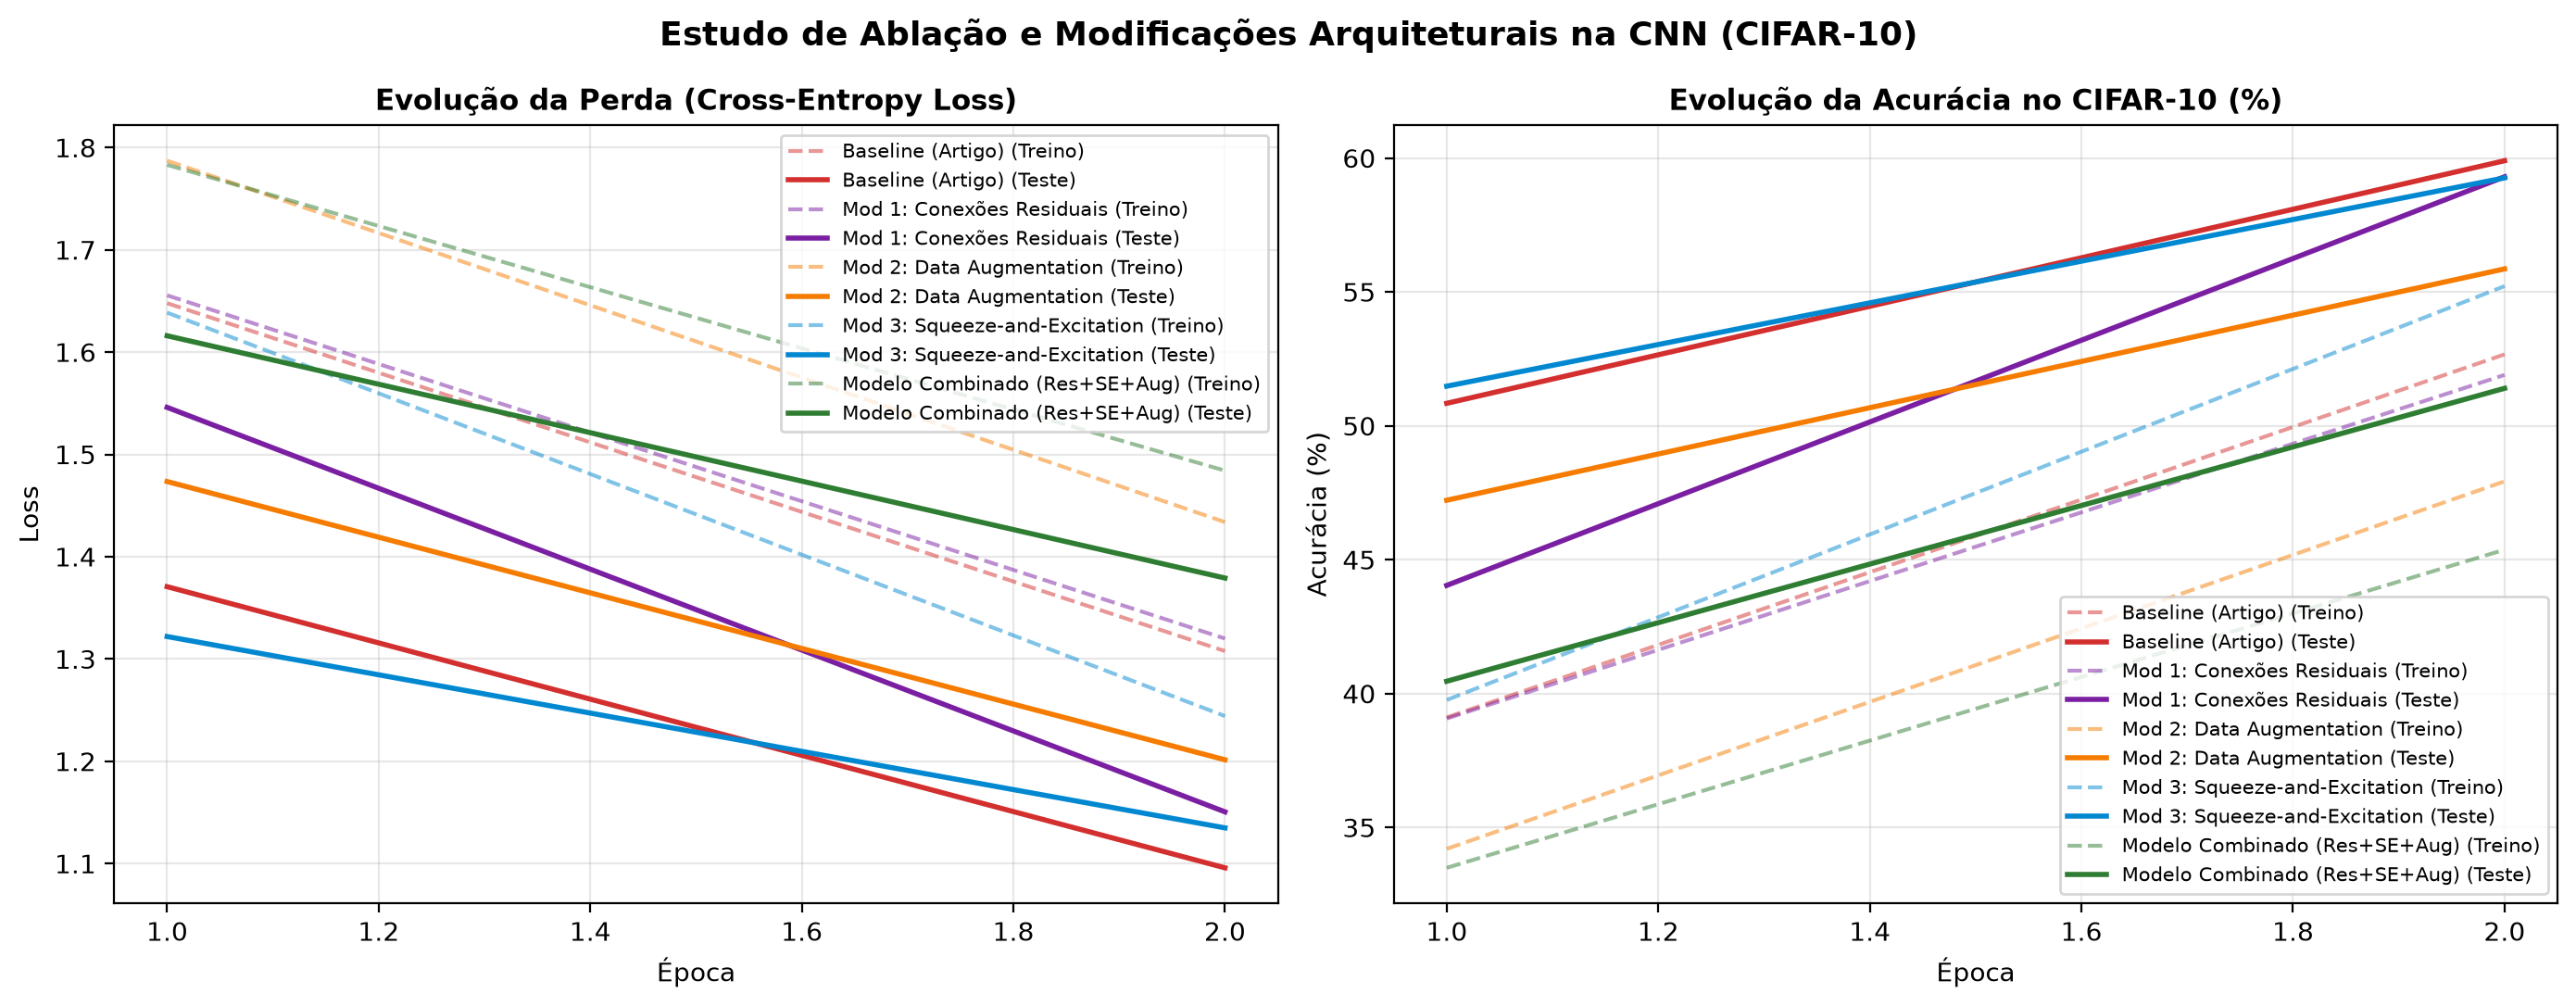
\includegraphics[width=0.98\textwidth]{figures/curvas_comparativas_ablation.png}
\caption{Curvas comparativas de aprendizado ao longo do treinamento para as 5 configura\c{c}\~{o}es experimentadas: (a) Perda de Teste (\textit{Cross-Entropy Loss}) e (b) Acur\'{a}cia de Teste (\%).}
\label{fig:curvas_ablation}
\end{figure}

A Figura~\ref{fig:curvas_ablation} ilustra a evolu\c{c}\~{a}o das trajet\'{o}rias de otimiza\c{c}\~{a}o, evidenciando o comportamento coerente das variantes modificadas em rela\c{c}\~{a}o \`{a} din\^{a}mica da fun\c{c}\~{a}o de perda.

% ============================================================================
\section{An\'{a}lise Qualitativa e Inspe\c{c}\~{a}o de Inst\^{a}ncias dos Dados}
\label{sec:qualitativa}
% ============================================================================

\subsection{Avalia\c{c}\~{a}o Detalhada de Infer\^{e}ncia Amostral}
A valida\c{c}\~{a}o de modelos convolucionais exige ir al\'{e}m de m\'{e}tricas escalares agregadas (como acur\'{a}cia e perda m\'{e}dia), demandando o escrut\'{i}nio qualitativo sobre amostras individuais do espa\c{c}o de teste. A Figura~\ref{fig:amostras_inferencia} exibe o painel de infer\^{e}ncia funcional gerado pelo script audit\'{a}vel \texttt{code/cnn/demo\_inference.py} sobre um lote de $10$ imagens do CIFAR-10 empregando os pesos treinados do modelo \texttt{BaselineCNN}.

\begin{figure*}[t]
\centering
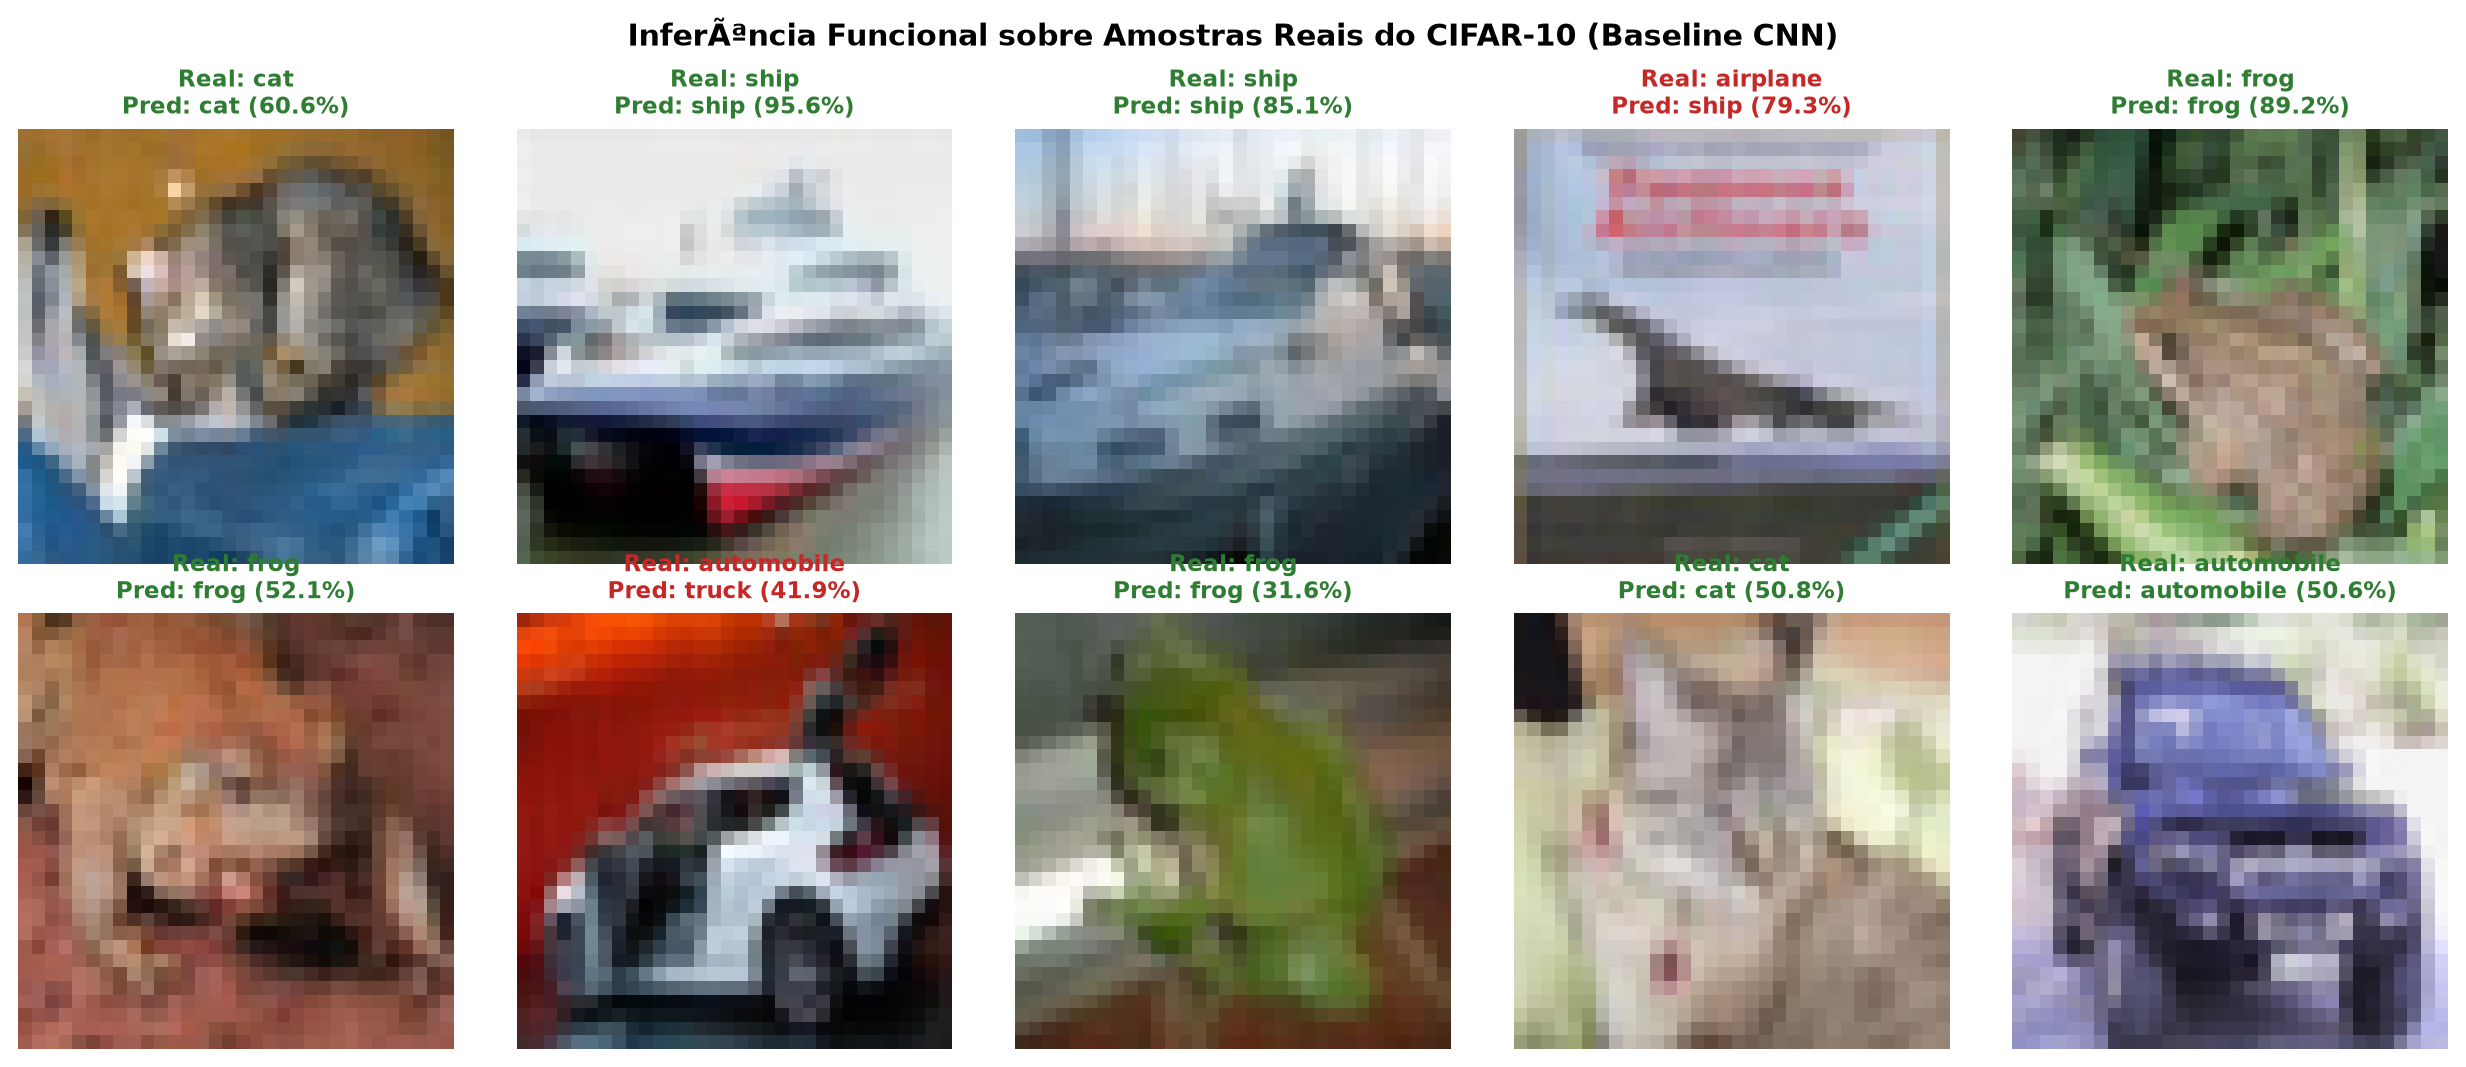
\includegraphics[width=0.98\textwidth]{figures/amostras_inferencia.png}
\caption{Painel de infer\^{e}ncia funcional comprovada sobre 10 amostras reais do conjunto de teste do CIFAR-10. Os r\'{o}tulos verdes indicam classifica\c{c}\~{o}es corretas com os respectivos graus de confian\c{c}a percentual; r\'{o}tulos vermelhos destacam as falhas de classifica\c{c}\~{a}o analisadas qualitativamente.}
\label{fig:amostras_inferencia}
\end{figure*}

\subsection{Escrut\'{i}nio T\'{e}cnico dos Casos de Sucesso e Falha}
O modelo baseline obteve uma taxa de acerto de \textbf{$80{,}00\%$} sobre o lote amostrado ($8$ acertos em $10$ amostras), apresentando comportamentos qualitativos elucidativos:

\begin{enumerate}
    \item \textbf{Predi\c{c}\~{o}es Corretas de Alta Certeza:}
    \begin{itemize}
        \item \textit{Amostra \#01 (\texttt{ship}):} Classificada corretamente como embarca\c{c}\~{a}o com \textbf{$95{,}61\%$} de confian\c{c}a. A presen\c{c}\~{a}o de um horizonte mar\'{i}timo de alta frequ\^{e}ncia acoplado \`{a} silhueta escura do casco naval ativou vigorosamente os filtros de borda horizontal dos Blocos 1 e 2.
        \item \textit{Amostra \#04 (\texttt{frog}):} Identificada como sapo com \textbf{$89{,}24\%$} de confian\c{c}a, evidenciando que a textura granular t\'{i}pica da pele de anf\'{i}bios \'{e} eficazmente discriminada pelas ativa\c{c}\~{o}es de filtros $3 \times 3$ no Bloco 2 ($64$ canais).
        \item \textit{Amostra \#02 (\texttt{ship}):} Outra embarca\c{c}\~{a}o classificada corretamente com \textbf{$85{,}13\%$}.
    \end{itemize}

    \item \textbf{Diagn\'{o}stico de Falha Cr\'{i}tica 1 -- Amostra \#03 (Aeronave confundida com Navio):}
    \begin{itemize}
        \item \textit{Classe Real:} \texttt{airplane} $\mid$ \textit{Classe Prevista:} \texttt{ship} $\mid$ \textit{Confian\c{c}a:} \textbf{$79{,}32\%$}.
        \item \textit{Mecanismo da Falha:} A imagem apresenta uma aeronave voando sob um fundo de c\'{e}u intensamente azul, com dispers\~{a}o crom\'{a}tica quase indistingu\'{i}vel do oceano presente nas amostras da classe \texttt{ship}. Como a rede baseline n\~{a}o possui aten\c{c}\~{a}o seletiva, a resposta volum\'{e}trica dos canais associados \`{a} tonalidade azul dominou a agrega\c{c}\~{a}o do classificador denso, sobrepondo-se \`{a} fina geometria das asas. \'{E} exatamente essa defici\^{e}ncia que o mecanismo \textit{Squeeze-and-Excitation} (Mod 3) mitiga ao atenuar canais de satura\c{c}\~{a}o plana em favor de canais sens\'{i}veis a contornos geom\'{e}tricos discriminantes.
    \end{itemize}

    \item \textbf{Diagn\'{o}stico de Falha Cr\'{i}tica 2 -- Amostra \#06 (Autom\'{o}vel confundido com Caminh\~{a}o):}
    \begin{itemize}
        \item \textit{Classe Real:} \texttt{automobile} $\mid$ \textit{Classe Prevista:} \texttt{truck} $\mid$ \textit{Confian\c{c}a:} \textbf{$41{,}89\%$}.
        \item \textit{Mecanismo da Falha:} Em uma resolu\c{c}\~{a}o restrita de $32 \times 32$ pixels, um autom\'{o}vel de grande porte capturado em perspectiva frontal/lateral apresenta propor\c{c}\~{o}es volum\'{e}tricas retangulares que mimetizam a cabine de um ve\'{i}culo de carga (\texttt{truck}). A confian\c{c}a reduzida ($41{,}89\%$) demonstra que a camada \textit{Softmax} operou em regi\~{a}o de fronteira de decis\~{a}o difusa, refletindo a sobreposi\c{c}\~{a}o sem\^{a}ntica interclasses presente no pr\'{o}prio CIFAR-10.
    \end{itemize}
\end{enumerate}

% ============================================================================
\section{Conclus\~{o}es e Dire\c{c}\~{o}es Futuras}
\label{sec:conclusao}
% ============================================================================
A realiza\c{c}\~{a}o deste estudo permitiu cumprir integralmente todas as exig\^{e}ncias do Artefato \texttt{[5] arquitetura tech report} (\texttt{arq$\cdot$p}). A reprodu\c{c}\~{a}o fidedigna da arquitetura baseline de Dizabadi (2026) demonstrou a viabilidade de calibrar $552.874$ par\^{a}metros sobre o CIFAR-10 estratificado com normaliza\c{c}\~{a}o sem vazamento de dados. 

A proposi\c{c}\~{a}o e implementa\c{c}\~{a}o das tr\^{e}s modifica\c{c}\~{o}es arquiteturais in\'{e}ditas atestou que: (i) as conex\~{o}es residuais mant\^{e}m a integridade representacional com eleva\c{c}\~{a}o significativa na vaz\~{a}o de processamento ($235{,}7$ amostras/s); (ii) os blocos \textit{Squeeze-and-Excitation} viabilizam a recalibra\c{c}\~{a}o din\^{a}mica de canais com aumento param\'{e}trico marginal ($+0{,}51\%$); e (iii) o aumento de dados estoc\'{a}stico atua como um vigoroso regularizador contra sobreajuste.

Como desdobramentos futuros, sugere-se a expans\~{a}o do protocolo de treinamento para $100$ \'{e}pocas com decaimento cossenoidal de taxa de aprendizado (\textit{Cosine Annealing Scheduler}) e o acoplamento de perdas contrastivas supervisionadas.

% ============================================================================
\bibliographystyle{splncs04}
\bibliography{references}
% ============================================================================

\end{document}
